\documentclass[12pt,fleqn]{article}\usepackage{../../common}
\begin{document}
Geometrik Anahtarlama ile En Yakın Noktaları Bulmak


Grafik, fiziksel simülasyonlarda pek çok sayıda obje 3 boyutlu ortamda dünyaya
salınıp, ayrı ayrı onlara fiziksel kurallar uygulanır ve nereye geldiklerine
bakılır. Bu hesap sırasında objelerin birbirine çarpıp çarpmadığını hesaplamak
gerekir fakat böyle bir hesap, eğer mesela $n$ tane obje var ise, her görüntü
karesinde her $n$ tane objenin her $n-1$ diğer objenin yakınında olup olmadığı
kontrolü anlamına gelir, ki hesapsal yük $O(n^2)$ olurdu. Eğer $n$ milyonlar ise
bu ağır bir yük oluştururdu.

Böleç tekniğini burada da kullanabiliriz. Öyle bir sihirli böleç fonksiyonumuz
olsun ki her kordinat için bir böleç değeri üretsin ve birbirine yakın
kordinatlar için bu değer aynı olsun. Böylece basit eşitlik kontrolü ile iki
kordinatın birbirine yakın olup olmadığını hemen anlayabilirdik. Tabii daha
detaylı kontrol için böleçleri aynı olan kordinatları daha detaylı teste tabi
tutardık, ama detaylı kontrolün yapılacağı obje sayısını çok daha azaltmış
olurduk.

Yerelliğe Hassas Böleç (Locality Sensitive Hashing, -LSH-)

Bu alandaki tekniklerden biri LSH tekniği. LSH ile çok boyutlu bir kordinate
sistemindeki noktaların yaklaşık olarak birbirine yakın olup olmadığını bölec
üzerinden hesaplayabiliyoruz. Tekniğin temeli rasgele izdüşümdür (random
projection). [3]'te anlatıldığı gibi rasgele izdüşümün ilginç bir özelliği
mesafeleri koruması, yani orijinal kordinate sistemindeki noktalar birbirine
uzaksa yansıtıldıktan sonra da uzak kalmaya meyilliler. 

Bunu herhangi bir (yani rasgele) 2 boyutlu düzlem üzerinde yansıtılan alttaki
noktalarda görebiliriz. Uzak olan noktalar duzlem uzerinde hala birbirine uzak.

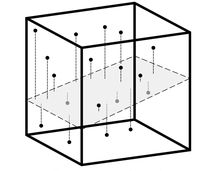
\includegraphics[width=10em]{algs_073_hash_01.png}

Tabii ki her (rasgele) düzlem her iki nokta arasındaki uzaklığı mükemmel olarak
göstermeyebilir. Fakat, eğer birkaç tane farklı düzleme yapılan yansımların bir
birleşimi olan bir ölçüt / bölec yaratabilirsek, o zaman bu ölçüt ile bazı hızlı
sonuçlara varabiliriz. 

\begin{minted}[fontsize=\footnotesize]{python}
vec1 = np.array([[-0.99137472, 0.61572851, -0.37733555, 0.0363575, -0.71647706]])
vec2 = np.array([[-0.16737788, 0.83147812, -2.06947369, -0.48174425, -1.60276846]])
vec3 = np.array([[-0.9074722, 0.75953396, 1.10696926, -0.8773451, -1.11589595]])

projections = np.array([[0.58834302, 0.24020825, 2.21323827, -0.21147486, 1.18477223],\
                        [-0.31146359, -1.88214137, -0.37489443, -0.58475914, -1.57121651]])
print (projections)
\end{minted}

\begin{verbatim}
[[ 0.58834302  0.24020825  2.21323827 -0.21147486  1.18477223]
 [-0.31146359 -1.88214137 -0.37489443 -0.58475914 -1.57121651]]
\end{verbatim}

\begin{minted}[fontsize=\footnotesize]{python}
print (vec1.shape)
print (np.dot(vec1, projections.T))
\end{minted}

\begin{verbatim}
(1, 5)
[[-2.12704963  0.39583023]]
\end{verbatim}


\begin{minted}[fontsize=\footnotesize]{python}
print (np.dot(vec1, projections.T) > 0)
print (  ''.join(((np.dot(vec1, projections.T) > 0)[0]).astype(int).astype(str))  )
\end{minted}

\begin{verbatim}
[[False  True]]
01
\end{verbatim}

\begin{minted}[fontsize=\footnotesize]{python}
print (  ''.join(((np.dot(vec2, projections.T) > 0)[0]).astype(int).astype(str))  )
print (  ''.join(((np.dot(vec3, projections.T) > 0)[0]).astype(int).astype(str))  )
\end{minted}

\begin{verbatim}
01
11
\end{verbatim}


\begin{minted}[fontsize=\footnotesize]{python}
def cosine_sim(vec1, vec2):
   return np.dot(vec1, vec2) / (np.linalg.norm(vec1)*np.linalg.norm(vec2))

print (cosine_sim(vec1[0], vec2[0]))   
print (cosine_sim(vec1[0], vec3[0]))   
print (cosine_sim(vec2[0], vec3[0]))   
\end{minted}

\begin{verbatim}
0.6524342023889728
0.5610062492540248
0.1169500241078299
\end{verbatim}

















Asal Sayılar ile Böleç (Hash) Tekniği

Böyle bir tekniği [1]'de görüyoruz. Teknik ile kordinat sistemini $l$
büyüklüğünde kutulara bölüyor, her eksen değerini bu büyüklük ile bölüyoruz,
bölüm sonrası elde edilen sayıyı taban (floor) tamsayıya indirgiyoruz, ardından
her eksen için farklı bir asal sayıyla çarpıp sonuçları XOR ile birleştiriyoruz
(ki XOR yaygın kullanılan bir böleç birleştirme yaklaşımı).

\begin{minted}[fontsize=\footnotesize]{python}
l = 5
n = 5
p1,p2,p3 = 73856093, 19349663, 83492791

x1 = [33,4,11]
x2 = [31,1,14]
x3 = [10,44,19]

def spatial_hash(x):
    ix,iy,iz = np.floor(x[0]/l), np.floor(x[1]/l), np.floor(x[2]/l)
    return (int(ix*p1) ^ int(iy*p2) ^ int(iz*p3)) % n

print (spatial_hash(x1))
print (spatial_hash(x2))
print (spatial_hash(x3))
\end{minted}

\begin{verbatim}
1
1
3
\end{verbatim}

Görüldüğü gibi ilk iki kordinat aynı böleç anahtarına düştü, ki bu iki kordinat
birbirine yakın.

Genel algoritma şöyle olabilir. Her görüntü karesi için iki faz düşünebiliriz,
ilk fazda tüm objelerin kordinat böleci hesaplanır, her böleç değeri altında bir
liste vardır, ve her obje anahtarının değerine tekabül eden o listeye
eklenir. İkinci fazda bir objeye bakarken onun üzerinde daha detaylı çarpışma
hesabı gerekip gerekmediğini anlamak için böleç anahtarındaki listeye bakarız,
listede sadece bir öğe var ise çarpışma yok, birden fazla ise o listedeki her
diğer obje için detaylı çarpışma hesabına devam edilebilir.

Bazi istatistikleri toplayalim. Acaba yaklasim ne kadar basarili?

\begin{minted}[fontsize=\footnotesize]{python}
from collections import defaultdict 
import numpy as np, datetime
import numpy.linalg as lin

mmin,mmax=0,400
p1,p2,p3 = 73856093, 19349663, 83492791
B = 500; L = 50; n = int(B/3)

def spatial_hash(x):
    ix,iy,iz = int(x[0]/L), int(x[1]/L), int(x[2]/L)
    tmp = (ix*p1) ^ (iy*p2) ^ (iz*p3)
    return tmp % n
    
balls = []
geo_hash_list = defaultdict(list)

for b in range(B):
    p = np.array([np.random.uniform(mmin,mmax,1)[0],
                  np.random.uniform(mmin,mmax,1)[0],
                  np.random.uniform(mmin,mmax,1)[0] ])
    balls.append({'pos':p, 'i': b})

for j,b in enumerate(balls):
    geo_hash_list[spatial_hash(b['pos'])].append(b)

tp = 0; tn = 0; fp = 0; fn = 0
for i,b1 in enumerate(balls):
    for j,b2 in enumerate(balls):
        if i==j: continue
        d = lin.norm(b1['pos']-b2['pos'])
        h1 = spatial_hash(b1['pos'])
        h2 = spatial_hash(b2['pos'])
        
        if d <= L and h1 == h2: tp += 1        
        elif d > L and h1 != h2: tn+=1
        elif d > L and h1 == h2: fp+=1
        elif d <= L and h1 != h2: fn+=1

print ('dogru pozitif', tp)
print ('dogru negatif', tn)

print ('yanlis pozitif', fp)
print ('yanlis negatif', fn)

print (tp+tn+fp+fn)
print ("Yanlis Negatif Yuzde %0.2f" % (fn / (tp+tn+fp+fn) * 100.0))
\end{minted}

\begin{verbatim}
dogru pozitif 456
dogru negatif 246340
yanlis pozitif 1340
yanlis negatif 1364
249500
Yanlis Negatif Yuzde 0.55
\end{verbatim}

500 tane topu rasgele bir şekilde her ekseni 0 ve 500 arasında olan bir uzaya
dağıttık. Topların bazıları yakın düştü tabii, bazılar düşmedi. Önce tüm topları
bölecledik ve sözlüğe koyduk. Sonra tüm topların birbiri ile olan mesafesini
ayrı ayrı teker teker külfetli yoldan yaptık, ve bölecin bu durum hakkında ne
söylediğine baktık. Pozitif bölec yakın diyor, negatif bölec uzak diyor
anlamında, tabii yakınlık ve uzaklık bölec anahtar değerinin aynı olup olmadığı
ile ölçülüyor.

Kontrolün doğru pozitif bulması mesela bölecin yakın dediğinin gerçekten de
yakın olması. Yanlış negatif tam tersi, bölec uzak diyor ama aslında toplar
yakın.

Tabii ki istediğimiz doğru hesapların değerlerin yüksek olması. Ayrıca
tekrarlayalım, bir simülasyonda işletirken yanlış pozitifin hala çaresi var,
bölecin yakın dediklerini bir kontrolden daha geçirirsek (problem değil o
noktada bakılan toplar azalmış oluyor, performans kaybı olmaz), bu kontrol
yanlış pozitifleri eleyecektir. Tek problem yanlış negatif, topların çoğu
birbirinden uzakta olduğu için bu yanlıştan dönmek zor, fakat bu tür toplar
yüzde 1'in altında.



















Kaynaklar

[1] {\em Optimized Spatial Hashing for Collision Detection of Deformable Objects}
    \url{https://matthias-research.github.io/pages/publications/tetraederCollision.pdf}

[2] Hari, {\em Locality Sensitive Hashing for Similar Item Search},
    \url{https://towardsdatascience.com/locality-sensitive-hashing-for-music-search-f2f1940ace23}

[3] Bayramli, {\em Rasgele İzdüşümü (Random Projection) ile SVD}

[4] Slaney, {\em Locality-Sensitive Hashing for Finding Nearest Neighbors},
    \url{https://www.slaney.org/malcolm/yahoo/Slaney2008-LSHTutorial.pdf}
    
\end{document}
